%\documentclass[acmtog]{acmart}
\documentclass[acmtog,anonymous,timestamp,review]{acmart} 
\usepackage{booktabs} % For formal tables
\usepackage[british]{babel}
\usepackage[utf8]{inputenc}
\usepackage{babelbib}
\usepackage{url}
\usepackage{graphicx}
\usepackage{subfig}
\usepackage{calc}
\usepackage{floatflt}
\usepackage{amssymb, amsthm}
\usepackage{amsmath}
\usepackage{tabularx}
\usepackage{multirow}
\usepackage{array}

\usepackage{xcolor}
\usepackage{bm}
\usepackage[normalem]{ulem}

\usepackage{stmaryrd}
\usepackage{stackrel}
\usepackage{algpseudocode}
\usepackage{algorithm}
\usepackage{rotating}

\usepackage{mwe,tikz}
\usepackage[percent]{overpic}
\usepackage{float}

\usepackage{pgfplots,pgfplotstable}

% Format source code
\usepackage{listings}
\usepackage{bm}
\usepackage{leftidx}

\usepackage[T1]{fontenc}
\usepackage{babel}
\usepackage[font=small,labelfont=bf,tableposition=top]{caption}
\usepackage{booktabs}
\usepackage{threeparttable}
\usepackage{multirow}
% graphics
\graphicspath{{figures/}{figures/}}

%{undoign silly float defaults}
\renewcommand{\topfraction}{0.8}	% max fraction of floats at top
\renewcommand{\bottomfraction}{0.8}	% max fraction of floats at bottom
\renewcommand{\dbltopfraction}{0.8}	% fit big float above 2-col. text
\renewcommand{\textfraction}{0.1}	% allow minimal text w. figs

\renewcommand{\floatpagefraction}{0.7}	% require fuller float pages
\renewcommand{\dblfloatpagefraction}{0.7}	% require fuller float pages

%Colors and plot structures
\newlength{\nbw}
\newcommand{\todelete}[1]{{\textcolor{red}{delete: #1}}}
\newcommand{\pc}[1]{\color{green}{#1}}
\newcommand{\nc}[1]{\color{red}{#1}}
\newcommand{\iname}{}
\newcommand{\sunq}{\color{blue}}
\newcommand{\changed}[1]{{\textcolor{orange}{#1}}}

\newcommand{\todo}[1]{{\textcolor{red}{TODO: #1}}}


\acmPrice{15.00}

% The next eight lines come directly from the completed rights form.
% You MUST replace them with the lines specific to your accepted work.
\setcopyright{acmlicensed}
\acmJournal{TOG}
\acmYear{2019}
\acmVolume{0}
\acmNumber{0}
\acmArticle{0}
\acmMonth{11}
\acmDOI{http://dx.doi.org/10.1145/8888888.7777777}

% Use the "authoryear" citation style, and make sure citations are in [square brackets].
\citestyle{acmauthoryear}
\setcitestyle{square}

% A useful command for controlling the number of authors per row.
% The default value of "authorsperrow" is 2.
\settopmatter{authorsperrow=4}

% end of preamble.

\begin{document}

% Title. 
% If your title is long, consider \title[short title]{full title} - "short title" will be used for running heads.
\title{End-to-End Complex Lens Group Design with Differentiable Ray Tracing}

% Authors.
\author{Qilin Sun}
\affiliation{%
  \department{Visual Computing Center}
  \institution{King Abudullah University of Science and Technology}}
\email{qilin.sun@kaust.edu.sa}

\author{Congli Wang(order dissuced by themself)}
\affiliation{%
  \department{Visual Computing Center}
  \institution{King Abudullah University of Science and Technology}}
\email{congli.wang@kaust.edu.sa}

\author{Qiang Fu(order dissuced by themself)}
\affiliation{%
  \department{Visual Computing Center}
  \institution{King Abudullah University of Science and Technology}}
\email{qiang.fu@kaust.edu.sa}

\author{Xiong Dun(order dissuced by themself)}
\affiliation{%
  \department{Visual Computing Center}
  \institution{King Abudullah University of Science and Technology}}
\email{xiong.dun@kaust.edu.sa}

\author{Wolfgang Heidrich}
\affiliation{%
  \department{Visual Computing Center}
  \institution{King Abudullah University of Science and Technology}}

% This command defines the author string for running heads.
\renewcommand{\shortauthors}{Qilin Sun, Congli Wang, Qiang Fu, Xiong Dun ,Wolfgang Heidrich}
\authorsaddresses{}
% abstract
\begin{abstract}
  
  Typical computational camera optics are usually manually designed for a specific 
  task and then combined with the correction work to post-capture possing. Recent 
  joint or end-to-end camera design still based on a separated design or using a 
  simple Fourier transform approximation and a single element.   
  
  
  However, limited by the designing freedom and overly approximation, the final 
  reconstructed image quality and robustness are still not good enough to step out
  of laboratory.
  
  
  In this paper, we propose an end-to-end designing architecture that jointly 
  optimizes a fully differentiable complex lens group with the reconstruction 
  algorithm. 
  Specifically, we build a differentiable complex lens representation based on 
  the differentiable ray-tracing rendering engine which enables directly 
  rendering intermediate images with aberrations of all kinds. 
  Skipping the PSFs, which vary across the field-of-view and depth, we 
  can now send the corrupted simulation into the reconstruction network 
  and correct the aberration described precisely.
  With a greater designing freedom and connection with the deep network, the 
  lens parameters and reconstruction can be directly optimized jointly 
  in the pipeline.
  
  
  We access the proposed method and its applications like extending
  depth-depth-of-field in both simulation and experimentally with a prototype camera
  system. The fully differentiable complex lens group can be a latent choice to replace
  Zemax and bring the optical engineering into a new epoch.
  
  
\end{abstract}

%CCS
\begin{CCSXML}
<ccs2012>
   <concept>
       <concept_id>10010147.10010371.10010372.10010374</concept_id>
       <concept_desc>Computing methodologies~Ray tracing</concept_desc>
       <concept_significance>500</concept_significance>
       </concept>
   <concept>
       <concept_id>10010147.10010178.10010224.10010226.10010236</concept_id>
       <concept_desc>Computing methodologies~Computational photography</concept_desc>
       <concept_significance>500</concept_significance>
       </concept>
 </ccs2012>
\end{CCSXML}

\ccsdesc[500]{Computing methodologies~Ray tracing}
\ccsdesc[500]{Computing methodologies~Computational photography}

%keywords
\keywords{Complex lens, Differentiable, Raytracing, End-to-end}

% A "teaser" figure, centered below the title and authors and above the body of the work.
\begin{teaserfigure}
  \centering
    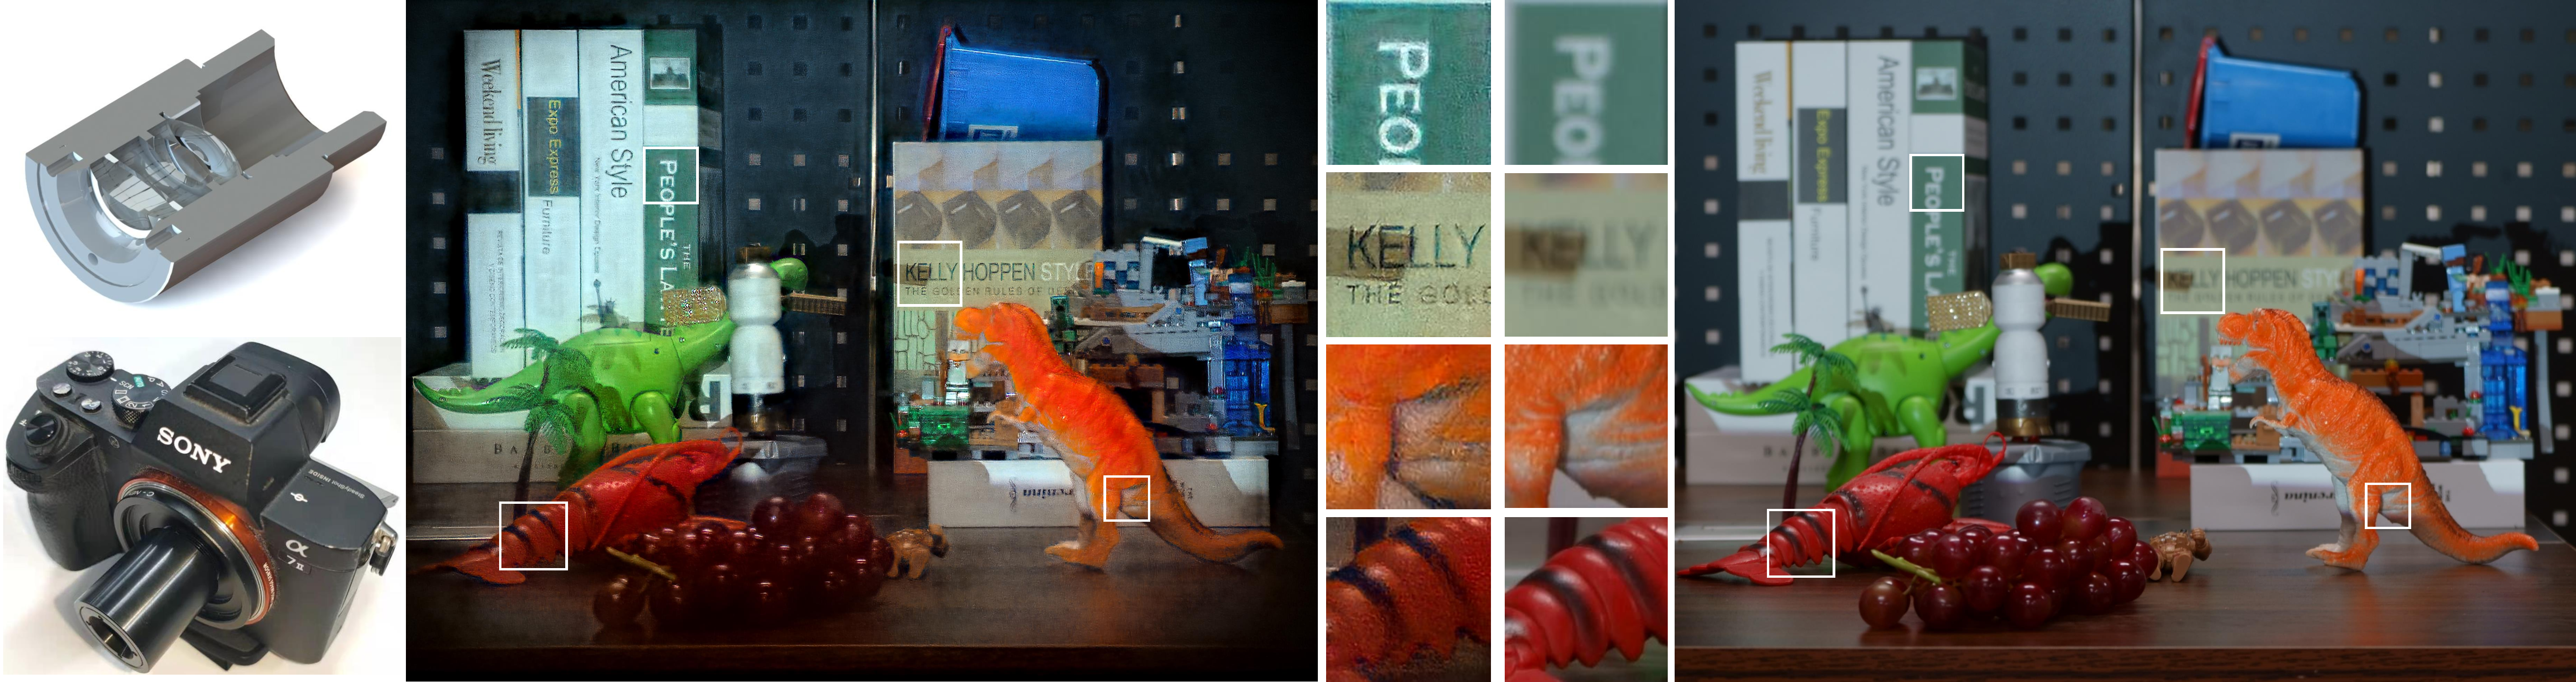
\includegraphics[width=1.0\textwidth]{figures/TeaserFigure.pdf}
    \vspace{-18pt}
  \caption{Overview of our 
\label{fig:teaser}}
\end{teaserfigure}

% Processes all of the front-end information and starts the body of the work.
\maketitle
%% introduction & related work
\section{Introduction}
\label{sec:intro}
 A camera, namely an optical instrument used to record images, was usually designed to acquire
 a sharper, higher dynamic range and better color fidelity image. 
 Therefore, in typical camera design, researchers take optical aberrations such as defocus, spherical  
 aberration, coma, astigmatism, field curvature, and distortion as the criterion to design optics. 
 As computing power grows, some optics designing software like Zemax and CodeV are developed to
 optimize the aberrations of all kinds. 
 However, this kind of design is mostly blindly pleasing human eyes but not the best for some
 specific tasks. 
 Facing a specific task, codesigning the optics and image processing~\cite{Sun2018Depth} even 
 end-to-end designings~\cite{Sun2020LearningRank1HDR} have emerged over the last two decades. 


 To date, codesiging of optics and the post-processing algorithm have achieved many new image 
 posiblities such as  depth estimation~\cite{Chang_2019_ICCV} large field-of-view 
 imaging~\cite{Peng_Sun2019LearnLargeFOV}, extended depth-of-field~\cite{chang2019deep}, optimal
 sampling~\cite{Sun2020EndSpad} and high dynamic range (HDR) 
 imaging~\cite{Sun2020LearningRank1HDR, Metzler_2020_CVPR}. 
 However, all those approaches are just variants of PSF engineering and very limited.
 First, for those diffractive based methods, the differentiable model is based on 
 paraximal approximation and simplified to a simple Fourier Transformation. The 
 small field-of-view, huge variable map, and difficult fabrication make the 
 applications very limited, hard to find a stable global minimum and large 
 scale application. 
 Second, for those refractive based methods, the optics and post-processing are still 
 optimized separately but not end-to-end. That means the optics is not optimal for
 the post-processing and always rely on prior knowledge.
 Last but not least, all those approaches fall to optimize the complex lens group like a
 traditional lens design. 

 In this work, we deviate from end-to-end design and traditional lens design goals and demonstrate 
 high-quality, large depth-of-field (DOF) imaging using a complex lens group with aspherical surfaces, 
 i.e., multiple lens surfaces which generate the best compromise for all depths connected with a 
 deep reconstruction network. Specifically, we propose a differentiable optical model with multiple
 elements and materials	which can be simply defined by a configuration file, a reconstruction deep
 network tailored to this optical model, and a novel loss and learning strategy that makes the
 end-to-end designing using our differentiable lens engine easier. 

 The differentiable complex lens model brings a new way to optimize the optic of many different kind
 of cameras. Combined with a tailored deep network, it makes it easier to recover high-quality images
 from measurements degraded by severe aberrations. Instead of traditional lens design, which usually
 taking point spread function (PSF) as a target, we are able to directly render the images with 
 abberations of all kinds. That means we can optimize the complex lens model without considering the 
 varying PSFs across the field of view and depths. In addition, beyond the goal of capturing a sharp
 and clear image on the sensor, the proposed method offer a huge designing flexibility that can not only
 find a compromision over optics and post-processing but also free the dimitions of optical encoding.
 We demonstrate the proposed approach outperforms the state-of-the-art complex lens design (by Zemax)
 in both simulation and experiment. We prototype our design camera with a complex lens by fabricating the
 CNC machining system that supports point diamond tunning and demonstrate on a broad set of experimental 
 in-the-wild captures. Our model is demonstrated more efficient in some given applications such as
 extended DOF compared with traditional lens design. In addition, we also show that the proposed
 differentiable complex lens model and end-to-end pipeline is effective in many other applications in
 simulation.
 
 Specifically, we make the following contributions:

\vspace{-3pt}
\begin{itemize}
\item We introduce a novel differentiable complex lens model based on differentiable ray tracing, and this model can simulate aberrations of all kinds. We provide an easy define of initial optics design that allows user to define aspherical surface profile, radius, positions, materials and etc..

\item We propose an end-to-end pipeline that can jointly optimize the lens model and the reconstruction network. With the reconstruction network and lose function which are tailored 
to some applications like extended depth-of-field. 

\item We validate the proposed approach in both simulations and on real-world measurements captured
by our assembled and fabricated aspherical lens group and verify that the experimental results match 
the simulations. 
\vspace{3pt}

\end{itemize}


 

\section{Related Work}
\label{sec:related_work}

\paragraph{Optical Aberrations and Traditional Lens Design.}
 The most common monocromatic abberations are defocus, spherical abberation, coma, astomatism, field
 curvature and distortation, and the cromatic abberations are typically axial and laterial chromatic
 abberation. Both of them are results of the differences of the optical path length when light travels
 trough different regions of a lens at different incident angles~\cite{fowles2012introduction}. These
 aberrations manifest themselves as unwanted blur which becomes more severe with increasing DOF~\cite{smith2005modern}. 
 Conventional lens design aims at minimizing aberrations of all kinds
by the tools like CODE V and ZEMAX who use . 
This includes designing aspherical surfaces and introducing lens elements using materials 
with different optical properties.

State-of-the-art optical design software is a cornerstone tool for optimizing
the surface profiles of refractive lens designs.
However, while hyper-parameter optimization tools are becoming mature, the design process still relies on existing objectives, so-called merit functions, that find a compromise across a variety of criteria~\cite{malacara2016handbook,shih2012image}, trading off the point spread function (PSF) shape across sensor locations, lens configurations (e.g. zoom levels) and target wavelength band. 
%Correcting all aberrations for a large FOV eventually results in a highly complex lens system.


\paragraph{Computational Optics.}
%
A large body of work on computational imaging~\cite{dowski1995extended,stork2013lensless,stork2014optical,levin20094d} has proposed to design optics for aberration removal in post-processing. %Commonly, these approaches favor PSFs that maximize the preserved spatial-frequency spectrum in at least one color channel, such that a deconvolution method can recover the missing frequencies effectively. 
These methods often favor diffractive optical elements (DOEs) over refractive optics~\cite{monjur2015ultra,antipa2018diffusercam,heide2016encoded,peng2016diffractive} because of their large design space. 
Moreover, recent work proposed caustic (holographic) designs, for projection displays or imaging lenses~\cite{papas2012magic,schwartzburg2014high,peng2017mix}.
To simplify the inverse problem in post-processing, all of the described approaches ignore off-axis aberrations by restricting the FOV to a few degrees -- {existing approaches do not realize monocular imaging with a large FOV}. 


Several approaches to end-to-end optical imaging were recently proposed, where parametrized optics and image processing are jointly optimized for applications in extended depth of field and superresolution imaging~\cite{sitzmann2018end}, monocular depth estimation~\cite{Haim:2018,Wu:2019,chang2019deep}, and image classification~\cite{chang2018hybrid}. However, none of these approaches aim at large FOV imaging and all of them build on simple paraxial image formation models, which break for large fields of view. Moreover, they are limited to a single optical surface. We overcome these challenges by engineering PSFs over a large FOV, and, relying on existing optical design tools that support complex multi-surface/material designs, optimize for a well-motivated dual-mixture design tailored to deep reconstruction models.



\paragraph{Manufacturing Planar Optics.}
%\todo{I don't think this characterization is accurate -- modern mobile
%camera lenses are all injection molded, which is the basically the
%same effort as nano-imprinting. The real hurdle to commercial
%adaptation is the software pipeline + chromatic aberration.}

Various manufacturing methods exist that enable ``planar'' optics with low-depth optical surface, i.e. less than 1~mm. 
Commercial miniature form factor optics like the lenses in smartphone cameras,
can be manufactured using mature injection molding techniques~\cite{oliver2010imaging}.
Alternative fabrication methods for thin-plate lenses include diffractive optics and metalenses~\cite{duoshu2011fabrication,genevet2017recent}, which require 
nano-fabrication methods like photolithography and nano-imprinting~\cite{ahn2009large,chou1996nanoimprint}. The UV-cure replication technique~\cite{zoberbier2009wafer} can facilitate manufacturing wafer-scale optical elements.
Note that creating a Fresnel lens with a clear aperture
  diameter of 23.5~mm and a focal length of 43~mm requires, as in this work, a feature size
  smaller than 300~nm, which is beyond the capability of the
  photolithography methods used in many recent DOE works~\cite{heide2016encoded,peng2016diffractive,sitzmann2018end}.
Freeform lenses with a larger aperture and continuous surfaces can be manufactured using diamond turning machining~\cite{fang2013manufacturing}. The continuous surface preserves light efficiency and works under broadband illumination, while the lenses are usually thick and bulky because of the local curvature constraints. 
%As a result, the size, cost, and image quality of existing lenses can not compete with complex compound lens systems.

In this work, we use high-precision diamond turning machining to prototype 
the proposed lenses. Instead of fabricating a 
freeform lens with continuous surface, e.g., as in~\cite{sitzmann2018end}, we wrap the optimized 
surface profile using coarse wrap-around depth values instead of wavelength-scale wrapping in diffractive lens designs, see Fig.~\ref{fig:teaser}. This allows us to design a Fresnel-inspired free-form lens with the advantages of both refractive optics and 
diffractive optics: we achieve a thin form factor while reducing chromatic aberrations.
%\gw{I don't think the arguments in this paragraph are clear. The fabrication part is not really a contribution of this work anyway, so why not omit this whole paragraph out and just list some of these implementation details in the implementation section later? }
%\fh{adjusted now, hope this makes sense. I think it's a minor contribution, so agree that this could be moved to the prototype section.}

\paragraph{Image Quality.}
Imaging describes the signal chain of light being transported from a scene patch of interest to the camera, focusing in the camera optics, digitization of the focused photon flux on the sensor, and post-processing of the measured data. During each of these individual steps, information about the scene patches of interest may be lost or corrupted. Various hand-crafted image quality metrics exist that measure the cumulative error of this imaging process~\cite{wang2004image,mitra2014denoise}, with or without known ground-truth reference~\cite{mittal2012no}, or allow to individually characterize components of the imaging stack using calibration setups~\cite{estribeau2004fast,emva1288}. Typical performance metrics are the signal-to-noise ratio 
(SNR)~\cite{parker2010algorithms} and modulation transfer function (MTF)~\cite{boreman2001modulation,estribeau2004fast}. While these metrics are widely reported and measurement setups are readily available, they are also not free from disadvantages due to their domain-agnostic design. For example, high SNR does not guarantee a perceptually pleasing image, which has sparked recent work on perceptual loss functions~\cite{johnson2016perceptual}. Moreover, SNR increases in the presence of glare and quantization, which can yield inconclusive results when used as a design metric~\cite{Geese_CDP}.

We design the proposed optical system in conjunction with the learned image reconstruction methods. To this end, we analyze the behavior of the early layers in our generator, which relate to the response of local contrast features in the scene. Relying on a probabilistic measure~\cite{Geese_CDP}, we assess the ability to detect or miss such local features across the full FOV.  This insight allows us  to tailor the proposed lens design to our network-based reconstruction method. 
 

\paragraph{End-to-end Optics Design.}
Codesigning of optics and post-processing has demostrated superior performance over some specific tasks in color image restoration~\cite{Chakrabarti2016LearningSM, Peng_Sun2019LearnLargeFOV}, HDR imaging~\cite{Sun2020LearningRank1HDR, Metzler_2020_CVPR}, single image depth estimation~\cite{Chang_2019_ICCV,Haim2018DepthEF, zhang2018single, He2018LearningDF }, microscopy~\cite{Horstmeyer2017ConvolutionalNN, kellman2019data, Nehme2019DenseTD, Shechtman2016MulticolourLM}, and spad camera~\cite{Sun2020EndSpad}.

We propose the differentiable complex lens model and embeded it to an end-to-end optimization pipeline.

Unfortunately, the lens design proposed in this work produces large PSFs that present a challenge to existing deconvolution methods which suffer in image quality for large aberrations, necessitating a custom image reconstruction approach.  Note that computationally efficient forward models for large spatially-varying convolutions have been investigated before~\cite{gilad2006fast}.

Over the last years, a large body of work proposed data-driven approaches for image processing tasks~\cite{Schuler_2013_CVPR,xu2014deep,
zhang132017learning}. Specifically addressing deconvolution, Nah et al.~\cite{nah2017deep} propose a fully connected convolutional network that iteratively 
deconvolves in a multi-stage approach. More recently, generative adversarial networks 
(GANs) have been shown to provide generative estimates with high image quality.
Kupyn \textit{et al.}~\cite{kupyn2017deblurgan} demonstrate the 
practicability of applying GAN reconstruction methods to deblurring problems.


All of these approaches have in common that they require either accurate PSF calibration or large training data that has been manually acquired. In contrast, we propose a lab capture process to generate a large training corpus with the PSF encoded in the captured data. Note that the large aberrations make training on very small image patches prohibitive. The proposed automated acquisition approach allows for supervised training on a very large training set of full-sized images, which are needed to encode large scene-dependent blur. The training approach, together with the proposed model and loss function, allows us to tackle the large scene-dependent blur, color shift and contrast loss of our thin-plate lens design. 


  

% --- DO NOT DELETE ---
% Local Variables:
% mode: latex
% mode: flyspell
% mode: TeX-PDF
% End:



%%
\section{Differentiable Lens Model}
\label{sec:optics}
As in most existing complex lens system,  the refraction are usually generated by either spericial lenses or asperical lenses.
Throughout the rest of this paper, we consider rotationally symmetrical lens profile designs which can be rotational symmetry facilitates manufacturing using turning machines.

In addition, our lens model can be easily applied to rotationally asymmetrical profiles like the expression 
of Zernik basis or even diffractive optics, and offer a new way to jointly optimize the refractive optics and diffractive optics.
\vspace{-3pt}
\subsection{Asperical Lens}
%
 The phase of a lens describes the delay of the incident wave phase introduced by the lens element, at the lens plane. The geometrical (ray) optics model, commonly used in computer graphics, models light as rays of photon travel instead of waves. 
%\fh{we should also visualize this. maybe Fig.~\ref{fig:optics_design} can be adjusted.} 
This model ignores diffraction, e.g. for light passing through a narrow slit. Although being an approximation to physical optics, ray optics still can provide an intuition: the perpendiculars 
%\gw{I don't think this word exists. please reformulate - not clear.}
%\fh{it's the noun version of the adjective perpendicular: https://dictionary.cambridge.org/dictionary/english/perpendicular} 
to the waves can be thought of as rays, and, vice versa, phase intuitively describes the relative delay of photons traveling along these rays to the lens plane, as illustrated with red lines in Fig.~\ref{fig:optics_design}. Hence, the phase of a thin lens is its height profile multiplied with the wave number and the refractive index~\cite{hecht1998hecht,goodman2005introduction}.  

 %We design the proposed lens system by optimizing a lens phase profile for a sparse set of on-axis and off-axis directions, corresponding to different focus areas on the image plane at different offsets from the image center. 
We design the proposed lens by first specifying an ideal phase profile
for perfect, spatially invariant PSFs over the full FOV, i.e., mapping
incident rays from one direction to one single point. Because it will
turn out intractable to manufacture this ideal lens, we propose an
aperture partitioning strategy as an approximation. The deviation of this
partitioned phase profile to the ideal profile is a
large low-frequency component which is independent of the incident
angle. Together with the peak-component, which preserves local
contrast over the full FOV, these two components make up the desired spatially invariant dual-mixture PSF. 

 To specify the ideal phase profile $\phi(r,\omega_i)$ for an incident ray direction $i$, and radial position $r$, see Figure~\ref{fig:optics_design}, we assume a physical aperture size $D$, focus distance $f$, and set: 

Aspheric lenses have been traditionally defined with the surface profile (sag) given by: 
\begin{equation}
\label{eq:sag}
Z(s) = \frac{cs^2}{1+\sqrt{1-(1+ \kappa )c^2s^2}} + \Sigma_{k=1} c_ks^{2k+2}
\end{equation}
%
 where $Z$ represents here is the sag of surface parallel to the optical axis,  $s$
 represents the radial distance from the optical axis, $c=1/R$ is the curvature or inverse of radius
 $R$. 
 $c_k$ represents the high order asperical coefficients. When the asperical 
 coefficients all set to zeros, the resulting lens surface becomes a conic $\kappa$.
 
 
 For  this  ideal lens profile, we define the output angle as:
%
 
\begin{equation}
\label{eq:targe_phase_2}
	\theta(r,\omega_i) = \mathrm{arctan} \left( \frac{\rho(\omega_i) - r}{f} \right),
\end{equation}
%
since the ideal lens design maps the incident rays from one direction $\omega_i$ to a single point with spatial position $\rho(\omega_i)$ on the image plane.

Next,  by inserting Eq.~\ref{eq:targe_phase_2} into Eq.~\ref{eq:targe_phase_1},  we derive the target phase $\phi$ as:
%
\begin{align}
%\begin{equation}
\label{eq:targe_phase_3}
%\begin{aligned}
\phi(r,\omega_i) &= -k \left[ r \cdot \mathrm{sin}\omega_i - \int_{0}^{r} \frac{\rho(\omega_i)-r_1}{\sqrt{f^2 + (\rho(\omega_i)-r_1)^2}} dr_1 \right] \\
&= -k\left[ r \cdot \mathrm{sin}\omega_i + \sqrt{f^2 +(\rho(\omega_i)-r)^2} - \sqrt{f^2 + \rho(\omega_i)^2} \right]. \nonumber
%\end{aligned}
%\end{equation}
\end{align}
%
 The ideal phase profile from Eq.~\ref{eq:targe_phase_3} is visualized
in Figure~\ref{fig:optics_design} (right). We observe a drastic
variation when approaching larger incident angles. In other words, the
same position on the lens aperture would need to realize different phases for
different incident angles, which is not physically realizable with
thin plate optics. 
%

 
\subsection{Aperture Partitioning}
%
Realizing the ideal phase profile is intractable to manufacture over the full aperture, as illustrated by the large angular deviations needed in off-axis region in Figure~\ref{fig:optics_design}.
To overcome this challenge,
we split the aperture into multiple sub-regions, and
assign each sub-region to a different angular interval, similar to prior work~\cite{levin20094d,zhu2013design} for refractive optics. 
 We note that this concept is also closely related to specializing optics depending on the incident ray direction in light field imaging~\cite{ng2005light}, for example, tailoring optical aberrations for digital correction~\cite{ng2012correction}. 
Specifically, we introduce a \emph{virtual aperture} $\mathcal{A}(r,\omega_i) =
circ[r-\mathrm{\nu(\omega_i)}]$ to partition the incident light bundle
of each direction into a peak component that we optimize for, while treating out-of-aperture 
components as out-of-focus blur. 
Here, $circ[\cdot]$ is a function representing a circular aperture, $\nu(\omega_i)$ indicates the axial center of the virtual
aperture subject to the $i^{\text{th}}$ incident ray direction. With this aperture partitioning, we optimize for the phase profile solving the following optimization problem: 
%we reasonably partition the incoming light bundle of each view into two components 
%Thus, our goal is to enforce a compromised high intensity peak of PSFs for all views, %we reasonably partition the incoming light bundle into two components. For this %purpose, we introduce a \emph{virtual aperture} $\mathcal{A}(x,\omega)=circle(x-d(\omega))$ and express the designing problem as the following optimization problem:    
\begin{equation}
\label{eq:lensOptim}
[\mathrm{\phi_0}(r),\mathrm{\rho},\mathrm{\nu}] = \mathop{\arg\min}_{\mathrm{\phi_0}(r),\mathrm{\rho,\mathrm{\nu}}}
\,\sum_{i=1}^{N} \|\mathcal{A}(r,\omega_i)(\phi_0(r)-\phi(r,\omega_i))\|_{2}^{2}. 
\end{equation}

Note that the virtual aperture is not a physical aperture
of the optical system, but is only  introduced as a conceptual partitioning in the lens optimization.
Figure~\ref{fig:float_aperture} shows the virtual apertures for uniformly sampled directions
superimposed on the real aperture.  For every direction, we optimize only
for the rays that pass through the  corresponding virtual apertures ; these
will be focused into a sharp PSF, while all other rays from the same
direction that miss $\mathcal{A}$ but pass through the full aperture
$D$ will be blurred and manifest as a low frequency ``haze'' in the measurement.

%% As we set constraints only on the \emph{virtual aperture}, the rays    %%
%% outside this aperture \emph{generally} considered out-of-focus,        %%
%% thereby can be reasonably assumed to form a large spot that is visible %%
%% as a low-frequency ''haze'' in the measurement.                        %%

%This is similar to the concept of aperture multiplexing but differs in that our virtual apertures have overlaps that we aim to compromise under a realistic effective aperture size.

 
\subsection{Fresnel Depth Profile Optimization} 
We solve the optimization problem from Eq.~\ref{eq:lensOptim} using
Zemax~\cite{geary2002introduction}.  While Eq.~\ref{eq:lensOptim} minimizes phase differences, Zemax interprets it as minimizing the optical path difference (OPD). 
Zemax allows us to piggy-back on a library of parameterized surface types, and directly
optimize a deep Fresnel lens profile ( a deeper micro-structure than regular 2$\pi$ modulation. ) instead of sequentially optimizing for the
phase and depth in a two-stage process.   We formulate the problem from Eq.~\ref{eq:lensOptim} using the multiple configuration function 
with the number of the configurations set to the discretized aperture directions (7 in this paper, uniformly sampled on half of the diagonal image size). We set the
size of each virtual aperture -- the effective aperture that contributes to focusing light bundles -- to one third
of the clear aperture.  As shown in
Figure~\ref{fig:float_aperture}, the center $\nu$ of the virtual
aperture for each direction along the clear aperture plane
can be modeled by shifting a stop along the optical
axis.  This allows us to optimize the location of the virtual aperture
by setting the stop position as an additional optimization
variable.  The merit (objective) function used in Zemax includes terms for
minimizing the wavefront (phase) error at each sampled direction, and
enforcing a desired effective focal length (EFL). 
We refer the reader to the supplementary document for additional details.

 
% 
\vspace{6pt}
\subsection{Aberration Analysis}
%
The optical aberrations of the proposed design have the following properties.
The chromatic variation is small because a deep Fresnel surface results in only small focal length differences in the visible wavelength region.
Off-axis variation (i.e. spatial intensity variation of PSFs 
across FOV) are small since we only control a part of light 
of each direction to focus into the sharp peak
(see Figures~2 and~7).

 
 
For each viewing direction, the PSF exhibits two components, a
high-intensity peak, which preserves local contrast, and a large
low-frequency component. We note that this property differs from 
 conventional spherical or aspherical singlets with the same
NA whose field curvature can be severe.  Although the low-frequency
PSF component reduces contrast, it does so
uniformly across the FOV.  In contrast to conventional single
  element optics, which have very poor contrast in regions far from
  the optical axis (required for wide-FOV imaging), it
  is this design which allows us to preserve the ability to detect
  some residual contrast, instead of completely losing contrast. 
%



%%
%\input{Evaluation}
%%
%\input{Implementation}
%
%\input{Conclusion}

\bibliographystyle{ACM-Reference-Format}
\bibliography{reference}
\end{document}



% --- DO NOT DELETE ---
% Local Variables:
% mode: latex
% mode: flyspell
% mode: TeX-PDF
% End:

